\section{Growth of non-axisymmetric modes without the influence of the
  planet}
%We first consider the linear stability of planetary gaps.  
In this section, the planet is introduced at $t=20P_0$ and 
its potential switched on over $10P_0$. At $t=30P_0$ we switch off the
planet potential and azimuthally average the surface density, energy
and velocity fields. At this point the planet has carved a partial
gap. We then perturb the density field and continue to 
evolve the disc. This procedure allows us to analyse the growth of
non-axisymmetric modes associated with the gap, but without
complications from non-axisymmetry arising directly from disk-planet
interaction.

Simulations were resolved with grid divisions of $(N_r,N_{\phi})=(1024,2048)$ with $r_{\mathrm{out}}=25r_{\mathrm{in}}$ for time up to $200P_0$ allowing high resolution and detection of high $m$ structures. Cases of $\tilde{\beta}=0.1,1.0,10.0$ were analyzed to provide a range of fast, moderate, and slowly cooled disks.

%The goal of these simulations is to compliment the disk-planet
%simluations presented later. 
These `planet-off' simulations are not linear stability calculations
since the cooling term in our energy equation restores the initial temperature profile corresponding to $H/r=0.05$, rather than the heated gap edge. Linear stability calculations and adiabatic cases will be further discussed in section~\ref{adiabatic_section}.

%disk-planet leads to heating 
%tcool tries to return it to the initial smooth profile (axisymmetric)
%if tcool > trwi -> temp returns to original value. heated gap not
%captured 

%There are two competing effects. Increasing
%$t_\mathrm{cool}$ leads to more heating and hence a larger sound-speed
%$c_s$, which favours instability \citep{li00} since the vortex
%instability is pressre-driven. However, gap-opening requires $r_h>H$,
%so increasing the sound-speed, and hence $H$, leads to a shallower
%gap (see below) and expected to be more stable. 

%tcool -> return to initial, t=0 temp. profile
%whereas the `basic state' is the gap profile with structured temp profile

%more details on perturbation: m=1 to 10, amplitude?  
%resolution?

\subsection{Gap structure}
%{\bf plots of the gap structure before instability sets in, e.g. at
%  t=30. surface density perturbation, gen. vortensity perturbation,
%  aspect-ratio. compare diff. beta. gaps become more shallow with
%  increasing cooling time (but not significantly - not enough time for
%  full gap formation). generalized vortensity: extrema smoothed out
%  with increasing cooling - expect more stability. aspect-ratio:
%  significant heating. increase in H so expect larger vortices
%}

Since stability of the gap is of interest we analyze the intial state formed by the planet-disk interactions. The intial gap profiles after the averaging procedure are shown in Fig \ref{intial1D} for varying $\tilde\beta$. Gaps formed are shallower for lower $\tilde\beta$ (faster cooling) but never significant enough to form a clear gap in this short timeperiod. Quicker cooling rates also result in steeper density gradients at the gap boundry and both the density maxima and density minima correspondingly increase and decrease with lower $\tilde\beta$. For all cases the gap width is $\approx 5r_{hill}$ which is set by torque balances in the disk \citep{crida06}.

 Generalized vortensity profiles show smoothening with larger cooling rates with the extrema becoming less pronounced. Charactereristicly for such disk-planet Rossby vortices the generalized vortensity minima correspond to density maxima in the disk. Larger $\tilde\beta$ values also as expected result in higher disk aspect ratios $H/r$, which is a value directly correlated to temperature in our model.

 For a planet to carve a gap in the surrounding material it has been shown that $q>H^3$ is needed \citep{crida06}. This indicates that for hotter disks, which have respectively higher $H$, it becomes more difficult by a cubic dependence for planet induced gaps to be formed. This is seen in our simulations as changes in $\tilde{\beta}$ result in changes of $h$ by less than $20\%$ yet gap depth almost doubles. Since generalized vortensity extrema are also correspondingly less pronounced and density gradients become smaller we expect that the stability of gaps to increase with larger $\tilde{\beta}$.

\begin{figure}
  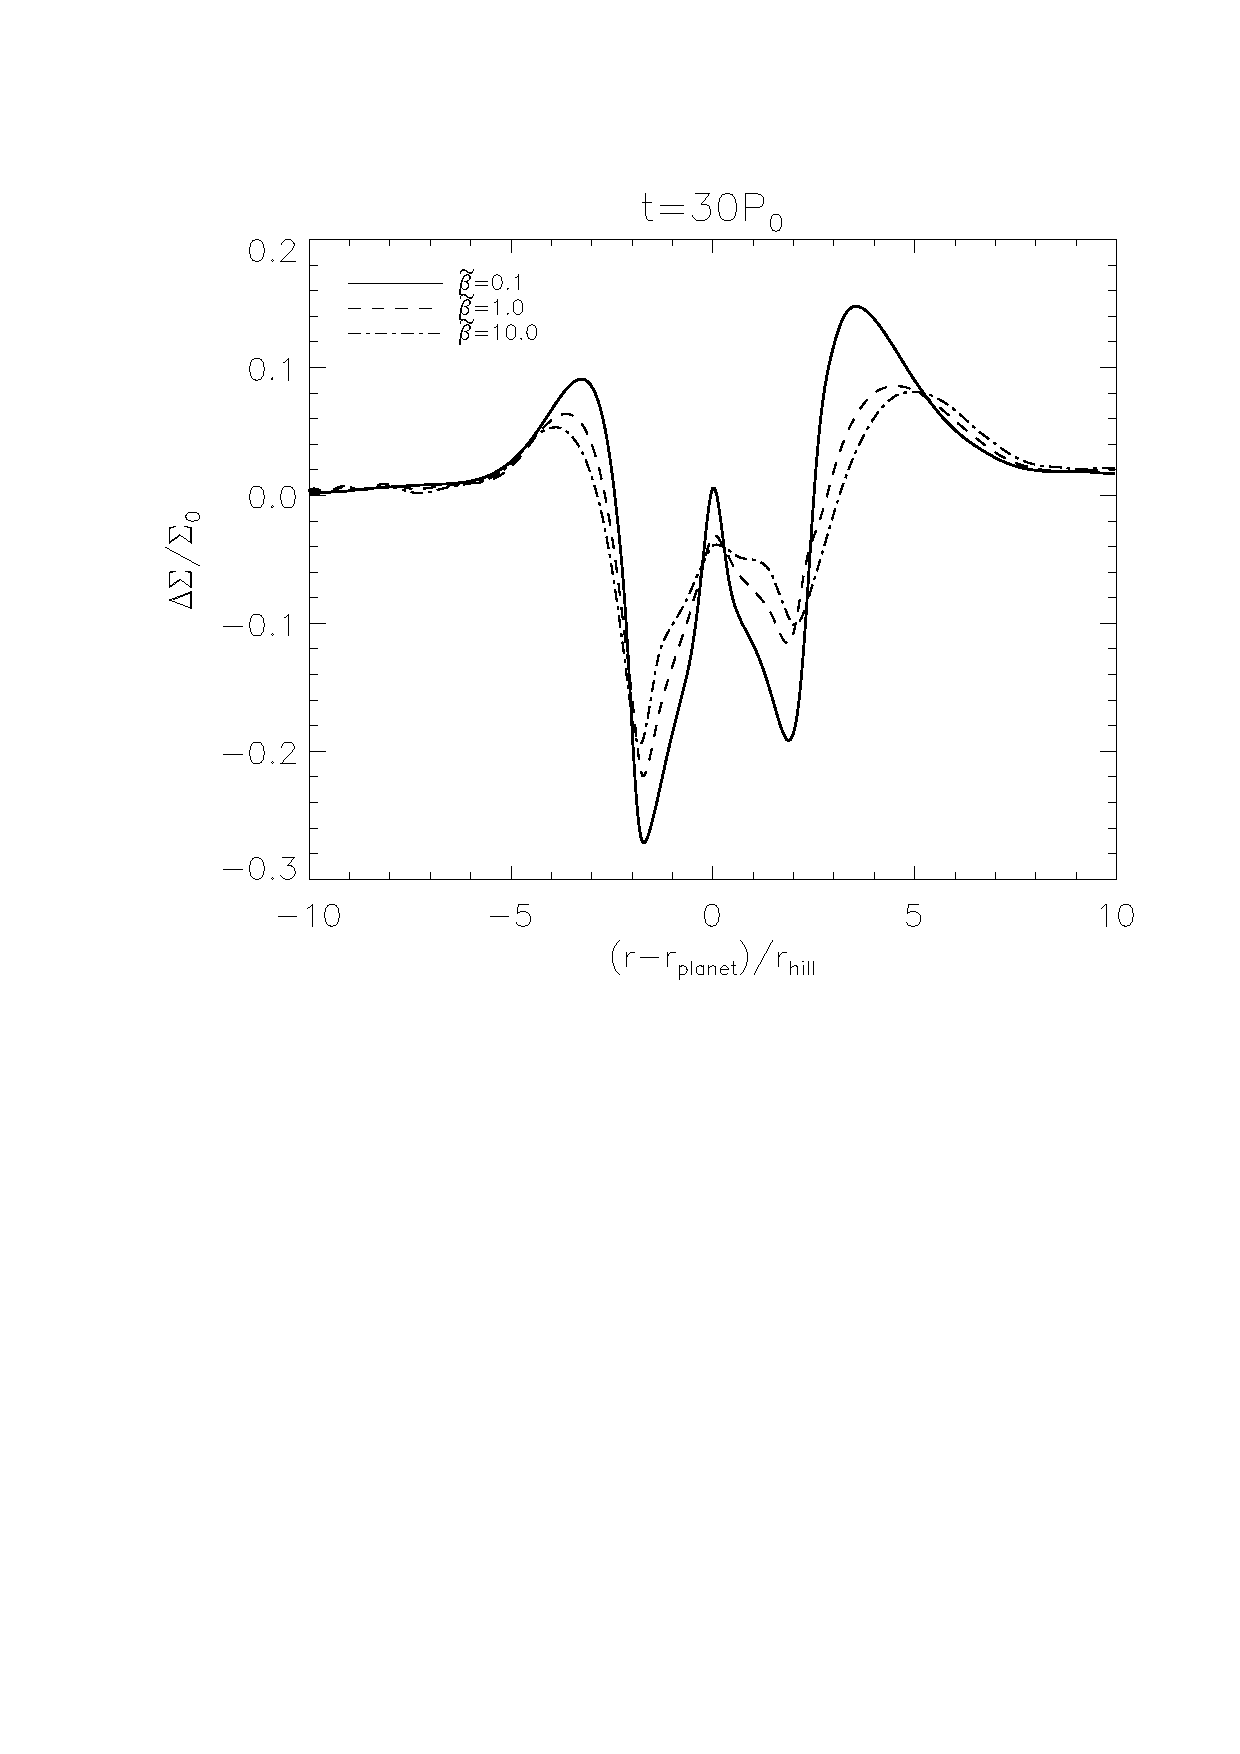
\includegraphics[width=.4\textwidth,clip=true,trim=0.5cm
    2cm 0cm 0cm]{figures/compare_sigma}
  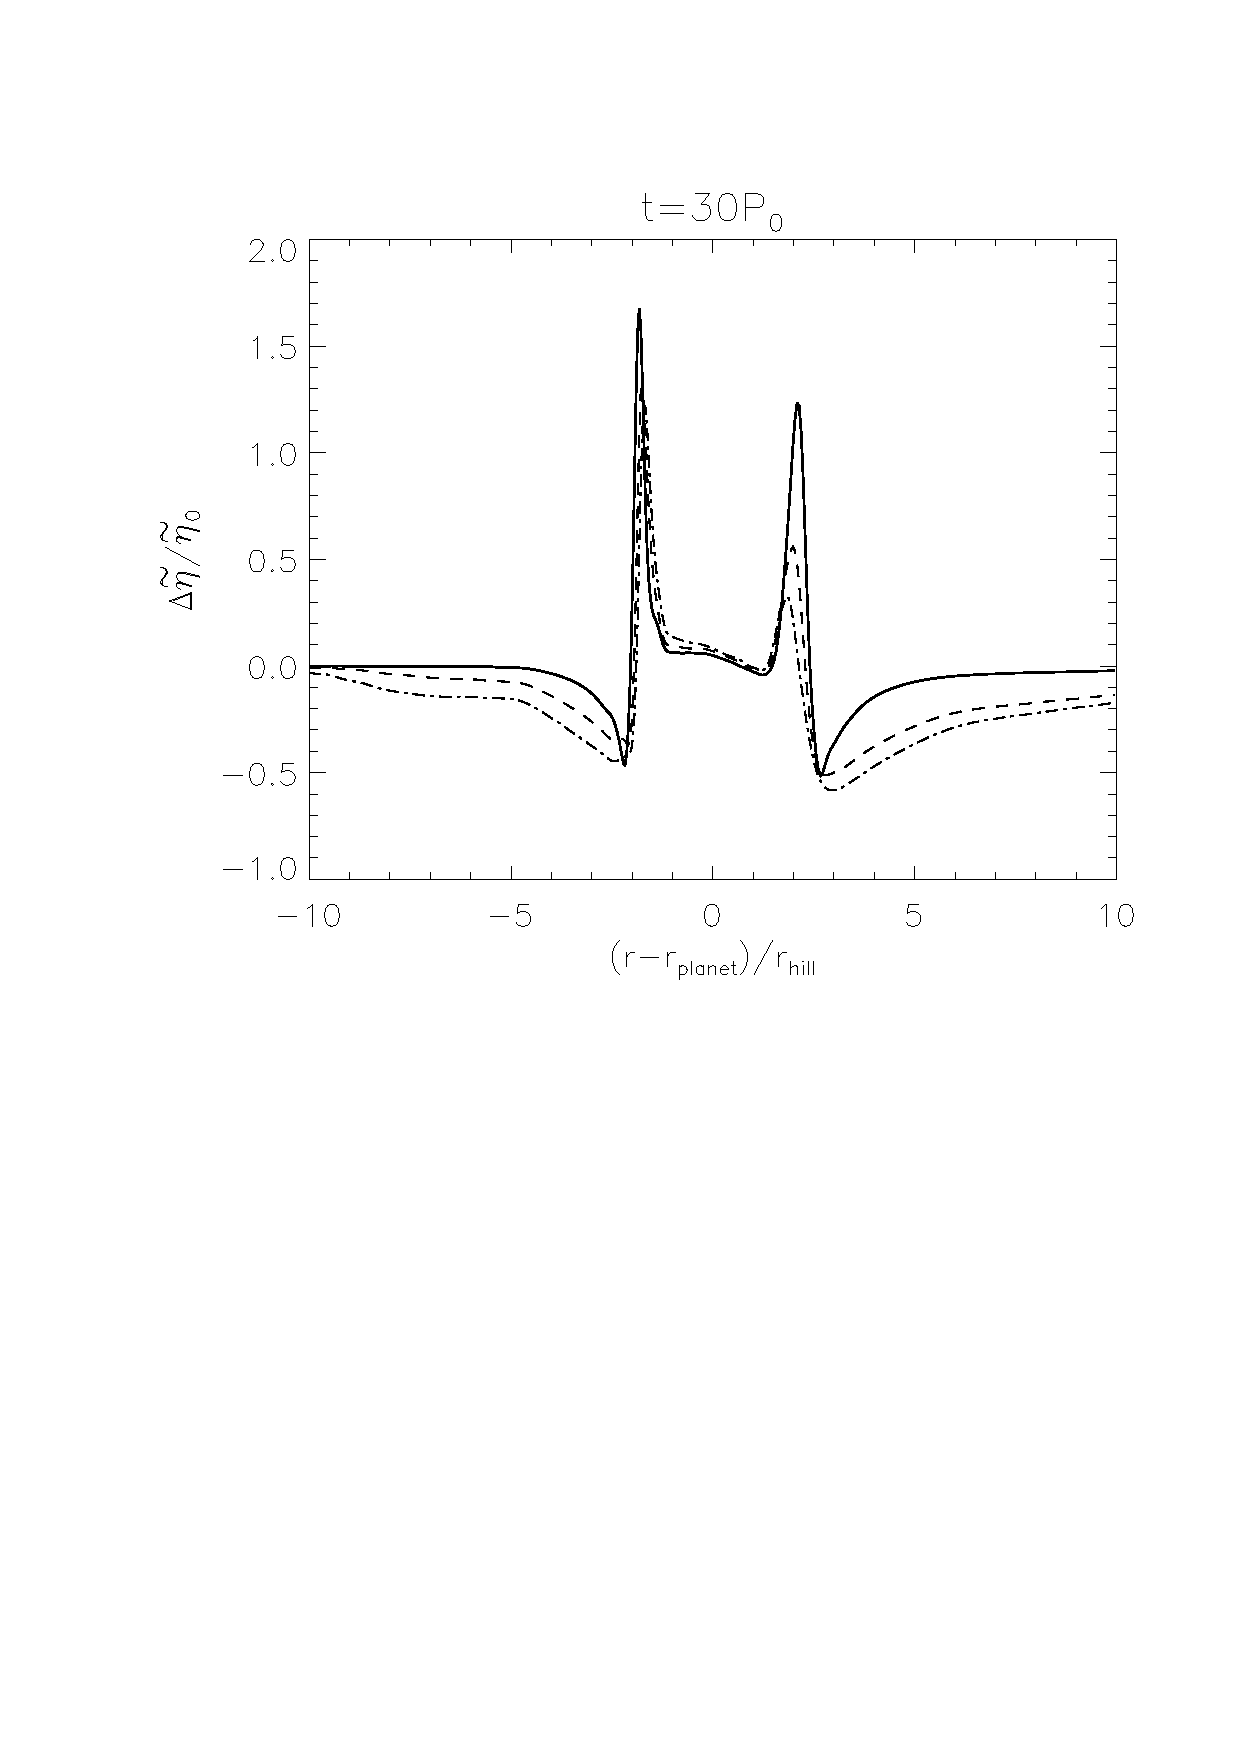
\includegraphics[width=.4\textwidth,clip=true,trim=0.5cm
    2cm 0cm 1cm]{figures/compare_gvortensity}
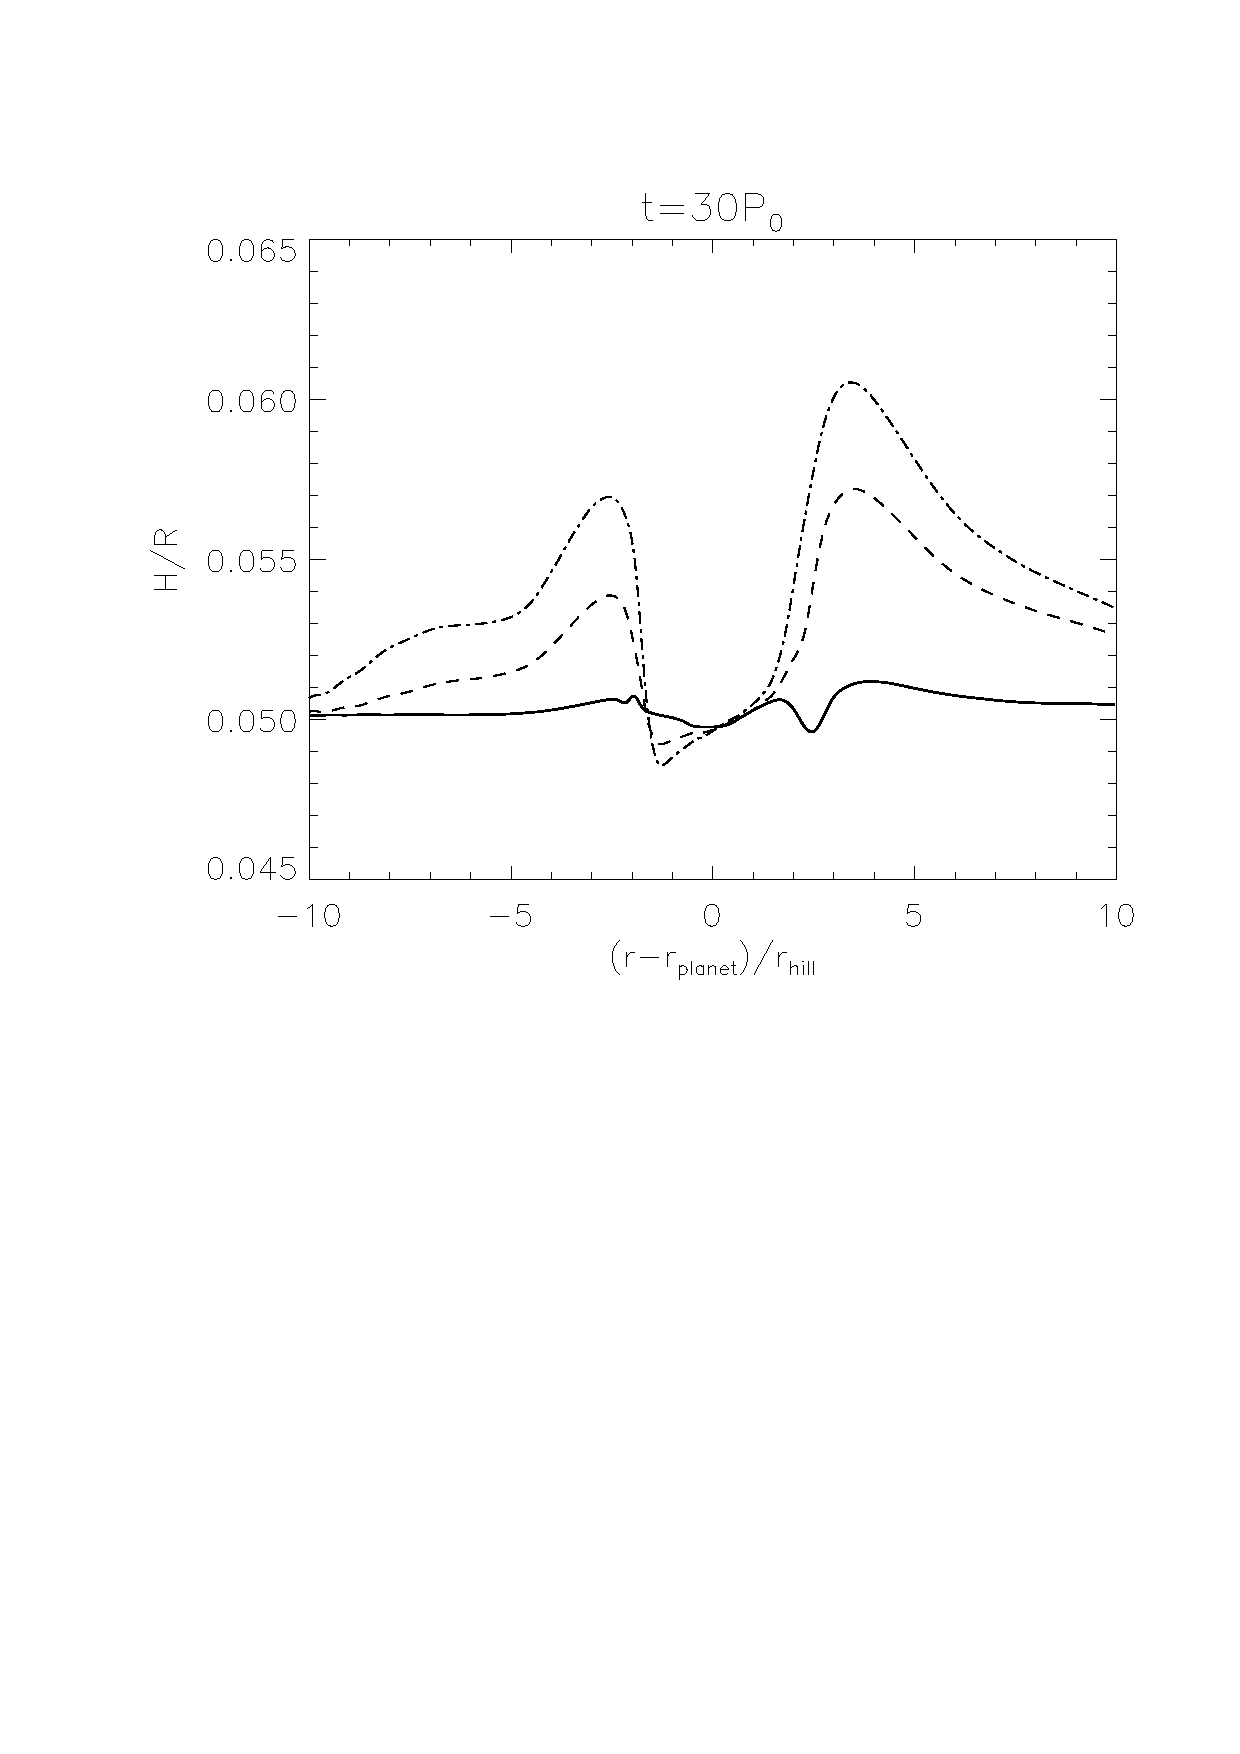
\includegraphics[width=.4\textwidth,clip=true,trim=0.5cm
    0.5cm 0cm 1cm]{figures/compare_aspectratio}
  \caption{Gap profiles at $t=30P_0$ for the intial partial gap opened before instability emerges for quick (solid line), moderate (dashed line), and slow cooling (broken line). Relative density pertibation (top), generalized vortensity pertibation (middle) and disk aspect ratio (bottom) are shown. \label{intial1D}}
\end{figure}


%\begin{tabularx}{0.4\textwidth}{l*{10}{R}} \toprule
%  \multicolumn{11}{c}{$\tilde{\beta}=0.1$} \\ \midrule
%  m                    & 1 & 2 & 3 & 4 & 5 & 6 & 7 & 8 & 9 & 10  \\ 
 % $\gamma10^2/\Omega(r_o)$ & 6.56 & 6.82 & 6.73 & 5.78 & 6.00 & 6.38 & 5.97 & 5.62 & 4.61 & 3.36   \\ \bottomrule
%\end{tabularx}

%\begin{tabularx}{0.4\textwidth}{l*{5}{R}} \toprule
%  \multicolumn{6}{c}{$\tilde{\beta}=1.0$} \\ \midrule
%  m                    & 1 & 2 & 3 & 4 & 5  \\ 
%  $\gamma10^2/\Omega(r_o)$ & 1.27 & 1.28 & 1.35 & 1.01 & 0.61   \\ \bottomrule
%\end{tabularx}

\begin{table}
  \centering
  \caption{Dominant mode and growth rates for $\tilde{\beta}=0.1,1.0,10.0$ (fast, moderate, and slow cooling) values during `planet-off' simulations \label{modetable}}
  \hfill
  \begin{minipage}{0.3\linewidth}
    \begin{tabularx}{\textwidth}{l R} 
      \multicolumn{2}{c}{$\tilde{\beta}=0.1$} \\ 
      \toprule
      m & $\gamma10^2/\Omega(r_p)$ \\
      \midrule
      6 & 7.3 \\
      7 & 7.8 \\
      8 & 7.9 \\
      9 & 7.9 \\
      10 & 6.8 \\ 
      \bottomrule
    \end{tabularx}
  \end{minipage}
  \hfill
  \begin{minipage}{0.3\linewidth}
    \begin{tabularx}{\textwidth}{l R} 
      \multicolumn{2}{c}{$\tilde{\beta}=1.0$} \\ 
      \toprule
      m & $\gamma10^2/\Omega(r_p)$ \\
      \midrule
      3 & 2.0 \\
      4 & 2.2 \\
      5 & 2.3 \\
      6 & 1.6 \\
      7 & 1.1 \\ 
      \bottomrule
    \end{tabularx}
  \end{minipage}
  \hfill
  \begin{minipage}{0.3\linewidth}
    \begin{tabularx}{\textwidth}{l R} 
      \multicolumn{2}{c}{$\tilde{\beta}=10.0$} \\ 
      \toprule
      m & $\gamma10^2/\Omega(r_p)$ \\
      \midrule
      1 & 1.1 \\
      2 & 1.6 \\
      3 & 1.7 \\
      4 & 1.2 \\
      5 & 0.1 \\ 
      \bottomrule
    \end{tabularx}
  \end{minipage}
  \hfill
\end{table}

\subsection{Linear modes and growth rates}\label{linear}
%{\bf present `planet-off' simulations. one `fourier mode v.s. time'
%  plot to show growth of linear instability. do an adiabatic case (or
%  extremely long cooling time) to see the effect of heated gap edge
%  (i.e. temp doesn't go back to t=0 value too quickly)
%  compare growth rate and dominant
%  m as function of beta (table). 2D figs to contrast (also used to
%  show it's the minimum in generalized pv that goes unstable.    
%  result: increasing cooling time makes the gap
%  more stable, and favors lower m. note: the `basic state' should be
%  the system at t=30 after azimuthal average. linear results should
%  have small perturbations. 
%}
After the azimuthal averaging, the small pertibation excites rapidly growing instabilities by the RWI. We analyticly charcterize these modes with quantities $m$ and $\gamma$ as defined by Eq.~\ref{fouriertransform} and Eq.~\ref{growth}. Table \ref{modetable} contains the results of the mode growth rates for a variety of cooling rates during this semi-linear phase. Results indicate that as $\tilde{\beta}$ was increased from $ 0.1\rightarrow10.0$ the dominant azimuthal Fourier mode decreased from $ m=9\rightarrow3$ and the respective growth rate decreased from $ \gamma/\Omega(r_p)=0.079 \rightarrow 0.017$. Snapshots of the instability in $r-\phi$ plane for the different $\tilde\beta$ are shown in Fig \ref{2Dlinear}.

These `planet-off' simulations, which are reminiscient of linear stability measurements, show that stability of gap edges increase with longer cooling rates (ie hotter gaps). This is as expected from the intial gap profiles and the gap forming criteria discussed in the previous section.

\begin{figure}
  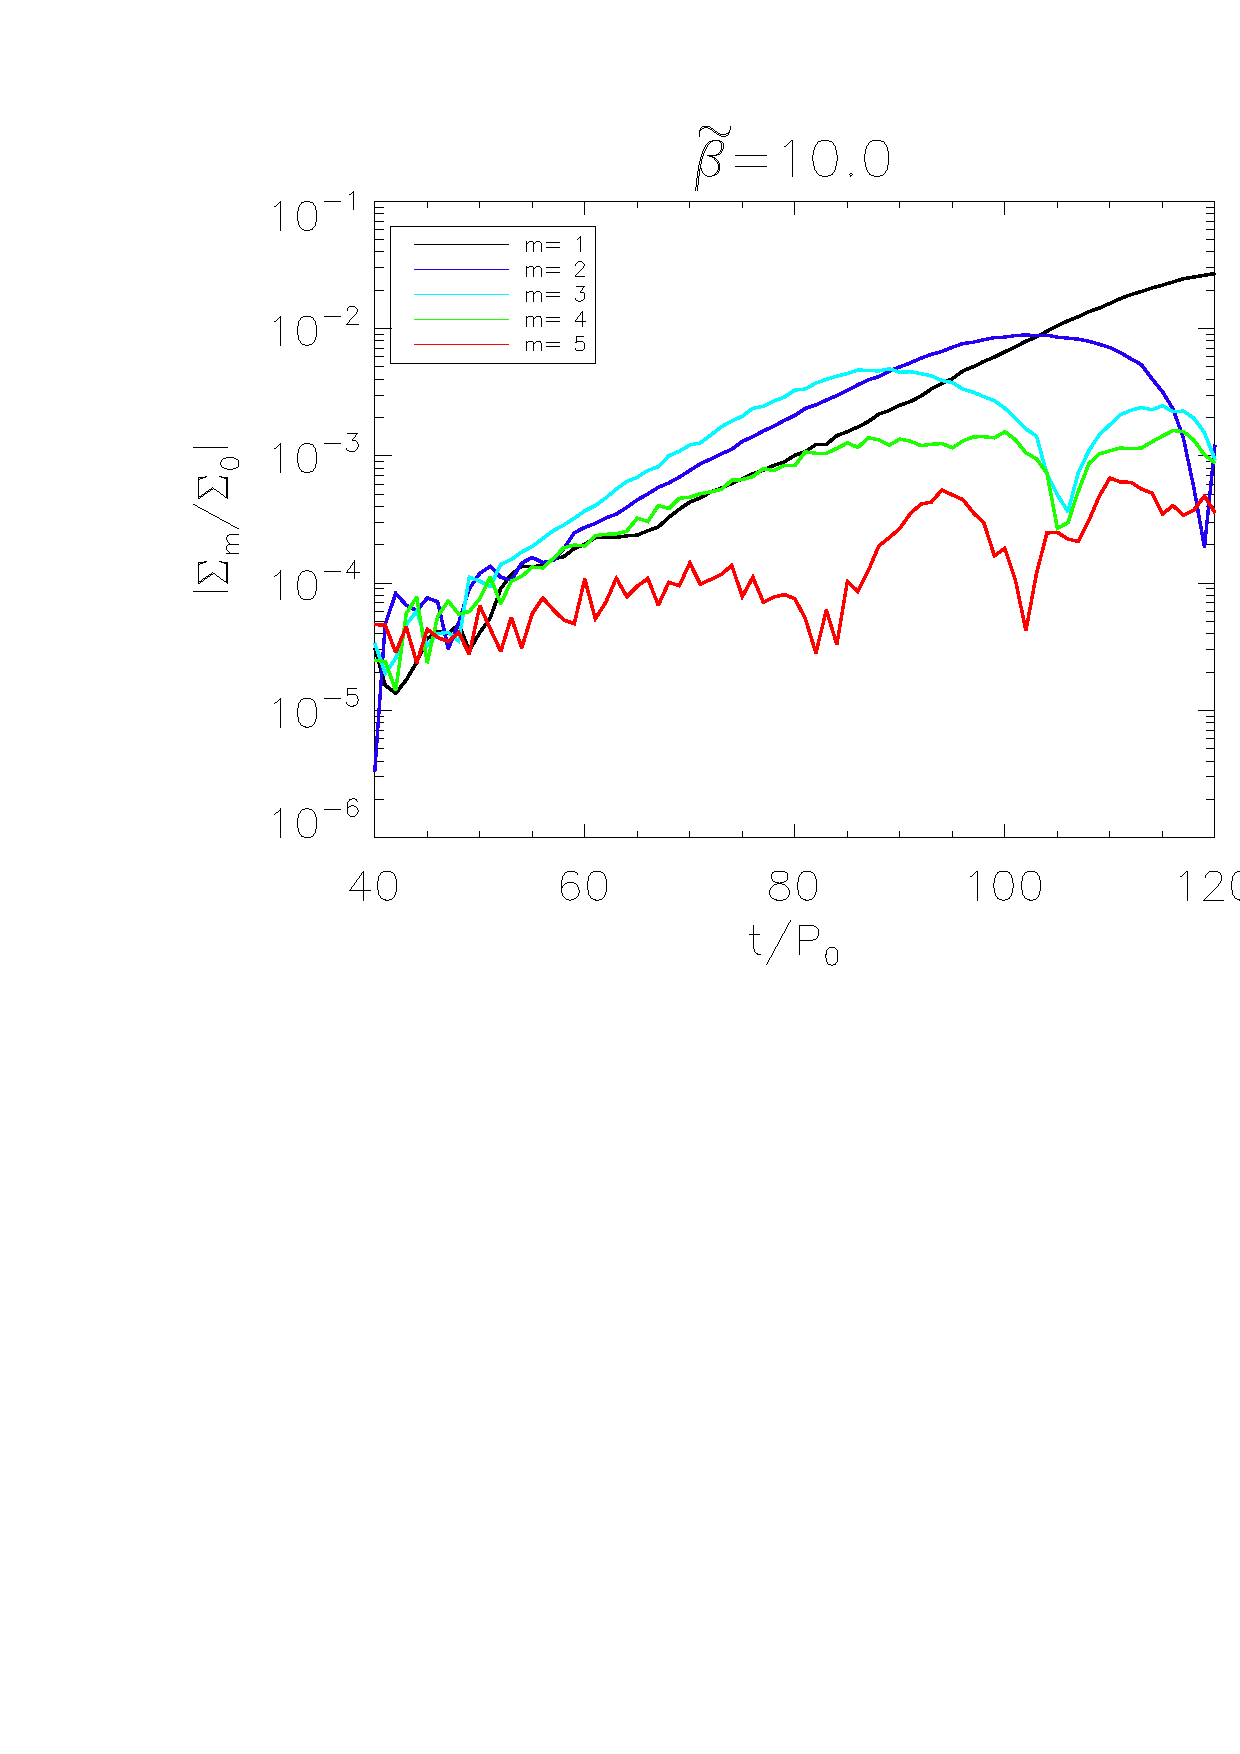
\includegraphics[width=\linewidth,clip=true,trim=1.2cm
    0cm 0cm 0cm]{figures/linear_stability}
  \caption{Log plot of the azimuthal Fourier modes of disk surface density non-dimenionlized by the background mode during the `planet-off' simulations for $\tilde{\beta}=10$. Colors correspond to different $m$ values. The $m=3$ component of the fourier transform is the fast growing mode during this growth phase of the instability and has corresponding $\gamma=0.017\Omega(r_p)$. \label{linearmodes}}
\end{figure}

\begin{figure*}
  \centering
  \subfigure{
    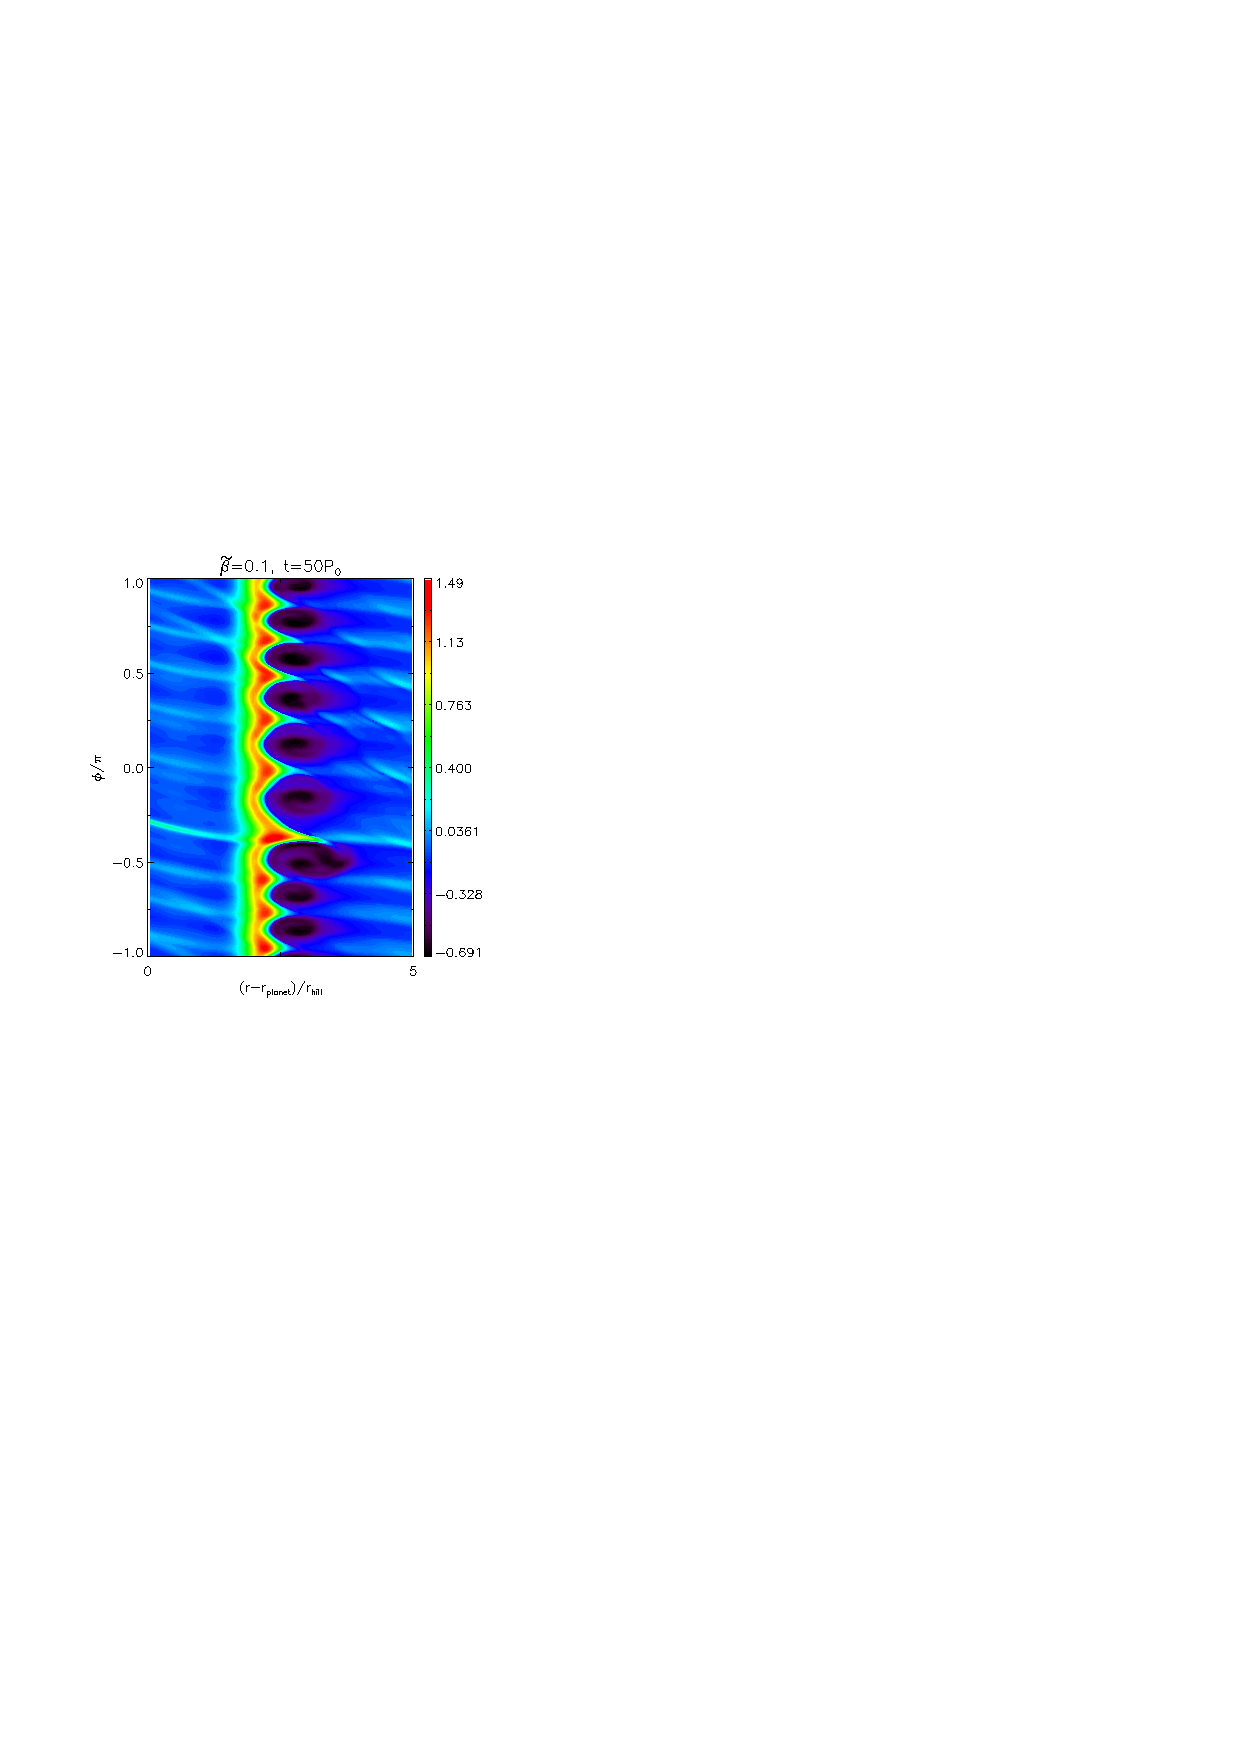
\includegraphics[width=0.3\linewidth]{figures/analysis_gvortensity_lowb}
  }
\hfill
  \subfigure{
    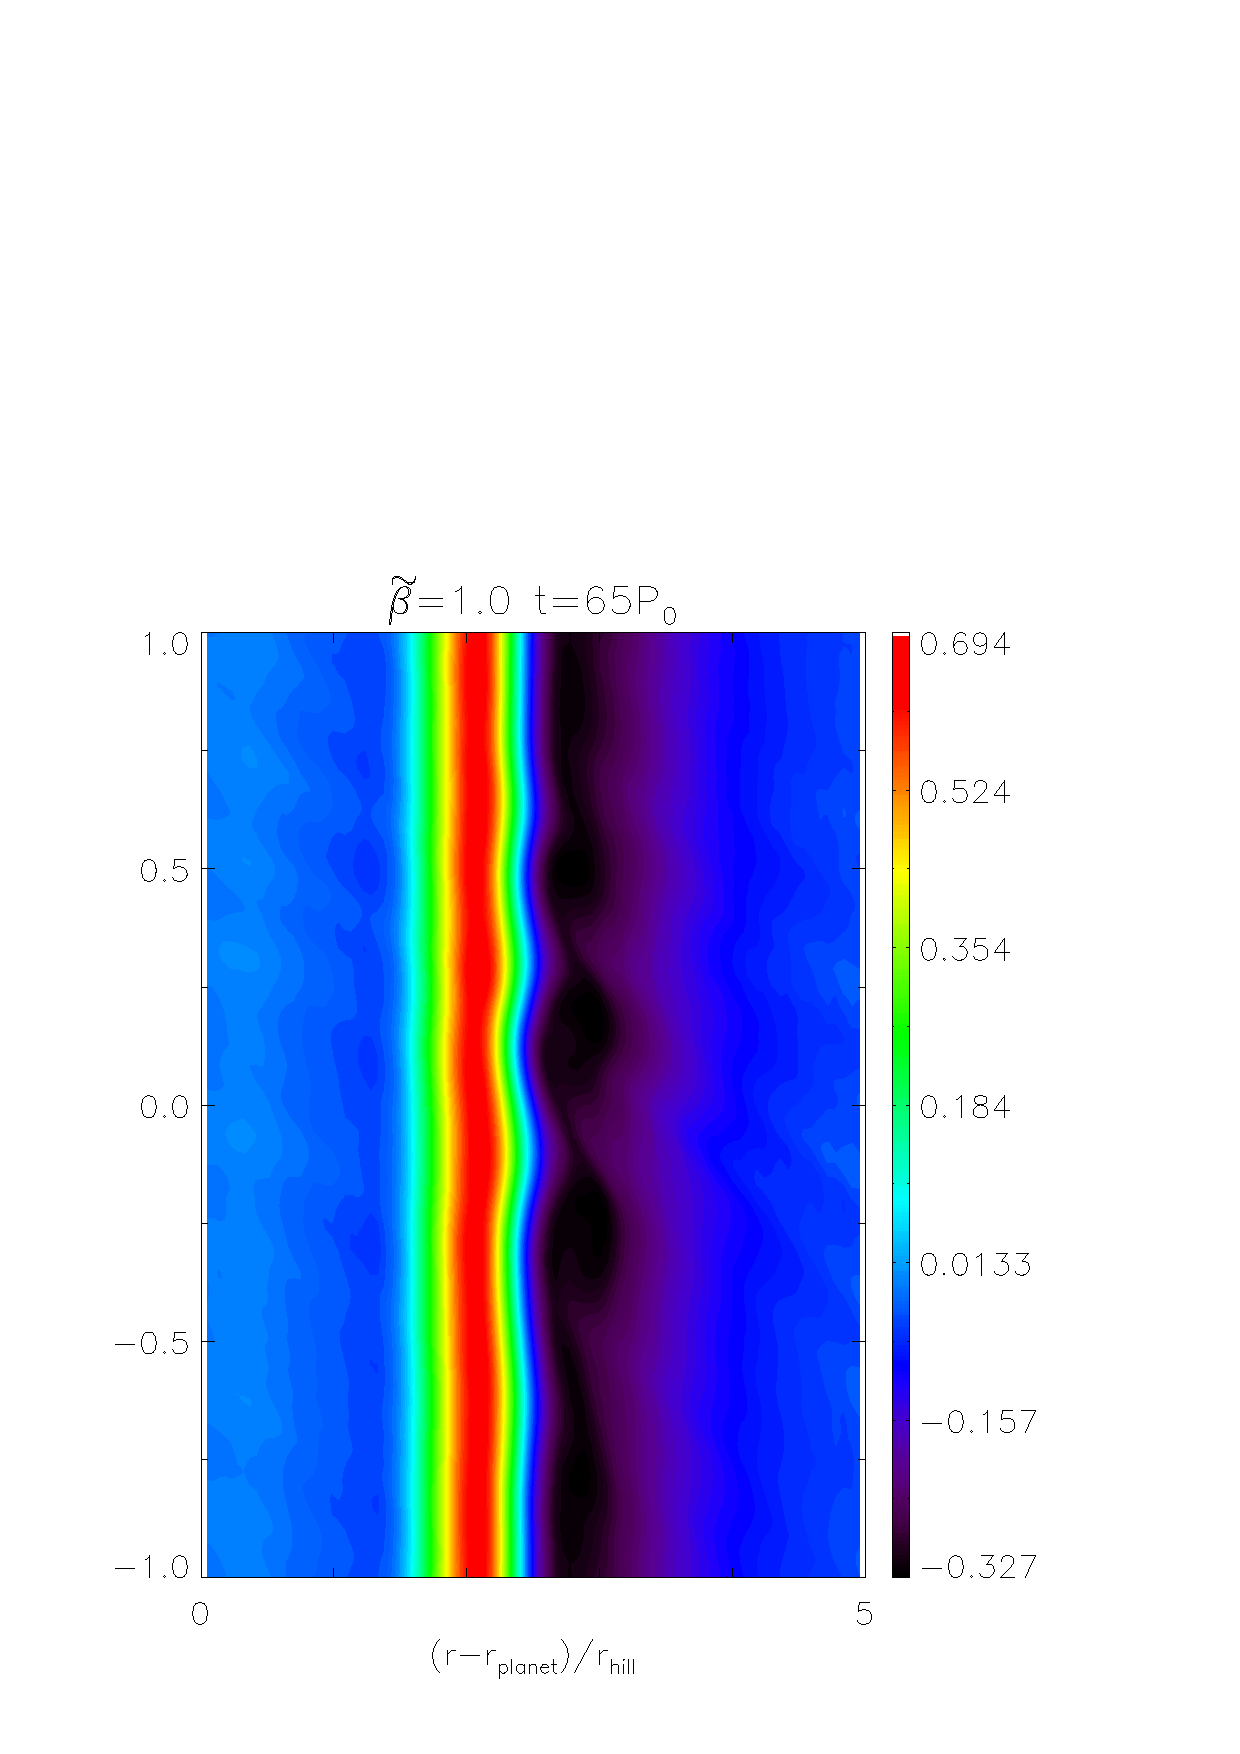
\includegraphics[width=0.3\linewidth]{figures/analysis_gvortensity_medb}
  }
\hfill
  \subfigure{
    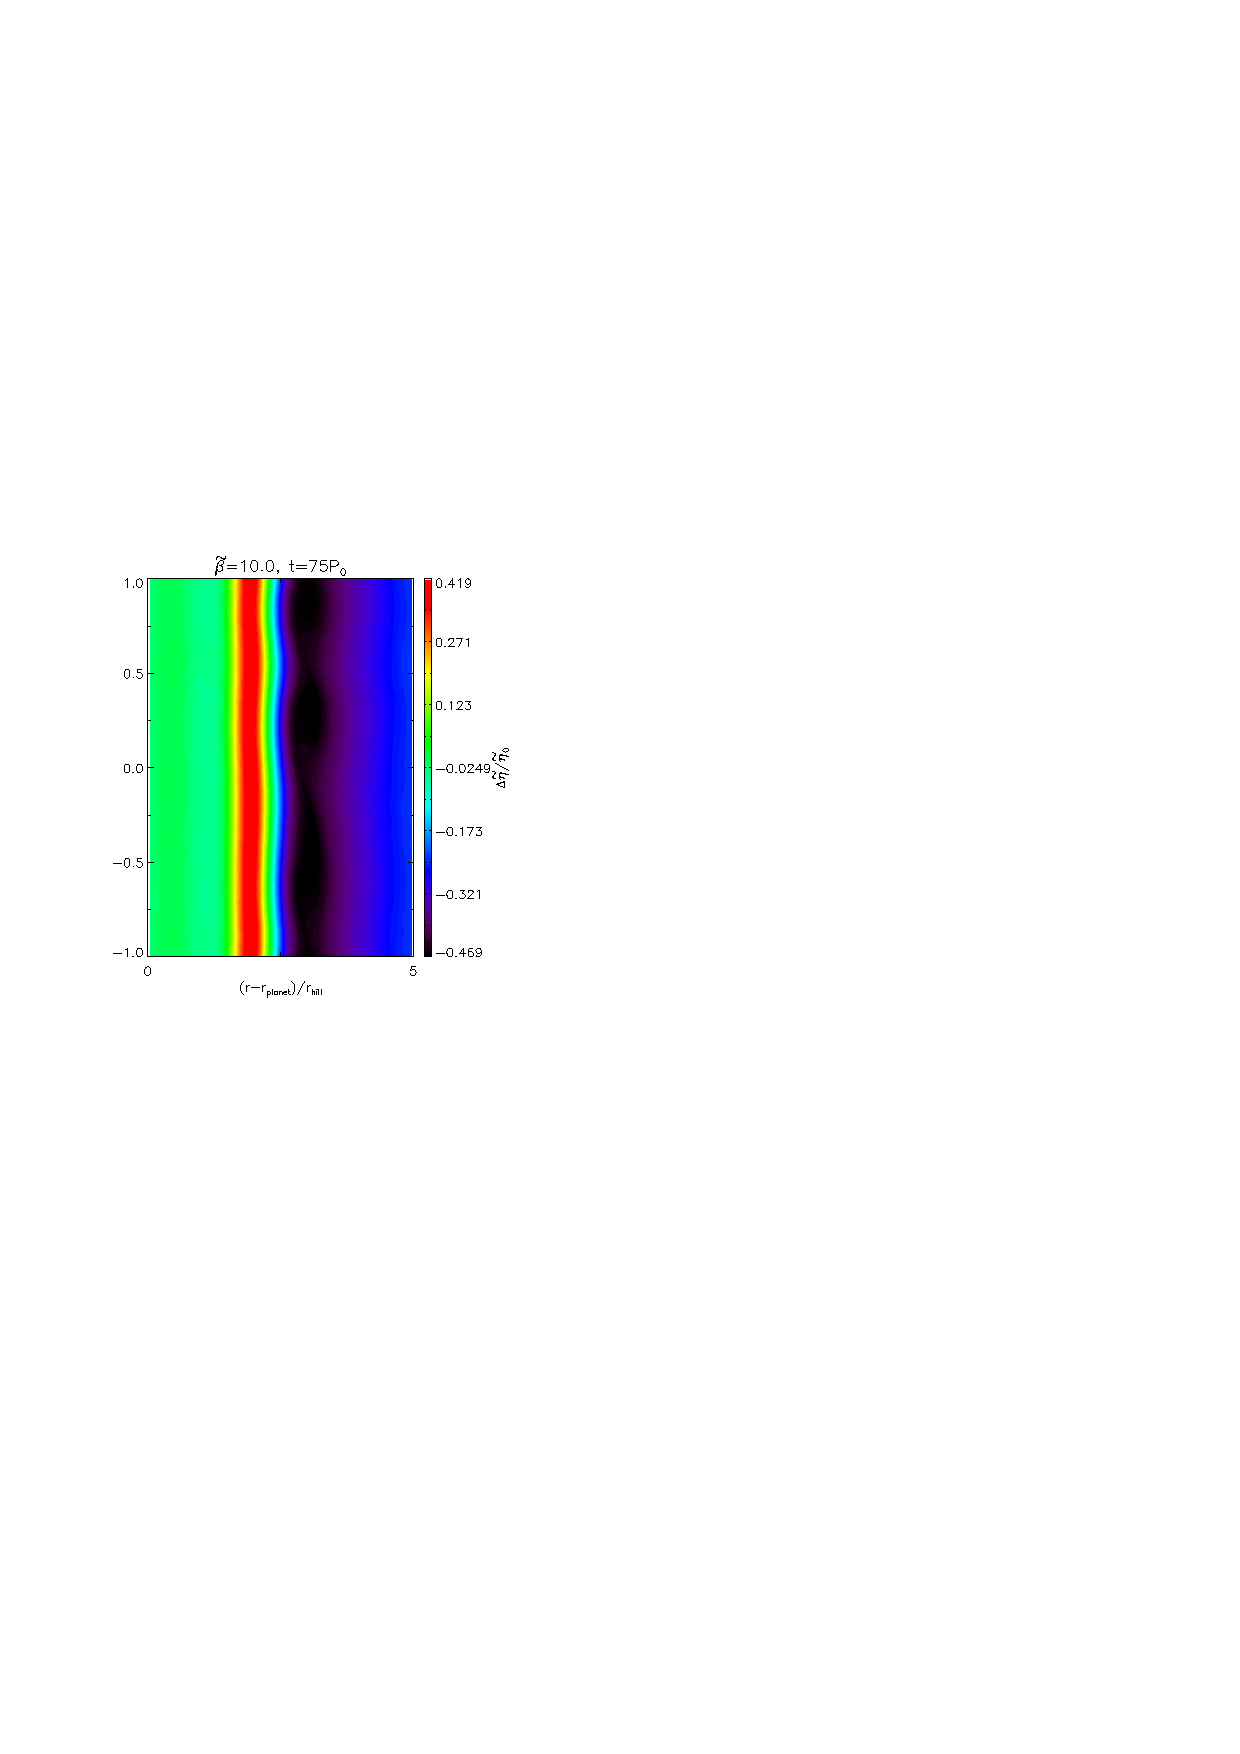
\includegraphics[width=0.3\linewidth]{figures/analysis_gvortensity_highb}
  }  
  \caption{Radial plots of the generalized vortensity pertibation for cases of $\tilde{\beta}=0.1,1.0,10.0$ (left,middle,right) during the linear phases of growth. The number of visible vortices decrease as $\tilde{\beta}$ increases and snapshot times correspondingly increase to capture the longer growth phases of the instabilities. \label{2Dlinear}}
\end{figure*}

\subsubsection{Nearly adiabatic disks}
\label{adiabatic_section}
%{\bf a case with extrmely long cooling time (or adiabatic run) in
%  order to look at effect of heated gap edge.  prelim result: not
%  important, at t=30, gap edge only heats to $H/r\simeq0.06$ even for
%  purely adiabatic disk. change in $h$ not important for linear
%  perturbations (but important for setting up the basic state). 
%}
During the `planet-off' simulations the analysis is not truly a linear stability measurement as we do not capture the effects of a heated disk on the instability growth. Since $t_{\mathrm{cool}}<t_{\mathrm{instability}}$ the disk manages to cool back to its intial value of $h=0.05$ before the instability emerges and thus we do not have a steady background state to form a linear stability problem. To compare our 'planet-off' analysis with a true linear stability analysis we ran a simulation  with $\tilde{\beta}=100.0$ which corresponds with an almost adiabtaic case. In this simulation the cooling rate is slow enough that the gap temperature profile changes only marginally over the timescale of the growth of the instability. The results show that the linear stability of the $\tilde{\beta}=100.0$ cases almost exactly equivilant to the case of $\tilde{\beta}=10.0$ in terms of mode growth rates and gap profiles. Since the disk heats up only to values $h\simeq0.06$ in the adiabatic case, the difference in growth rates between this and the original disk temperature of $h=0.05$ changes almost insignificantly as shown by linear theory \citep{li00}. This indicate that a continuously hot gap edge is not as important for development of vortices as the heating effects on the formation of the intial gap state.

%% We first describe results for weakly self-gravitating
%% discs $Q_0=8$ (giving $M_d=0.015M_*$) so that the gap remains 
%% gravitationally stable \citep{lin11b}. We also impose a dimensionless
%% kinematic viscosity $\hat{\nu}=2\times10^{-5}$ to suppress the Rossby
%% vortex instablity \citep{valborro07}. These parameter values
%% are typical for disc-planet simulations and yield stable/steady 
%% gap profiles. This will be useful reference cases to  
%% understand the unstable cases considered later.  

%% Fig. \ref{lvisc_steady_gap} shows the steady state gap profiles in terms of the relative
%% surface density and aspect-ratio at $t=200P_0$. Three levels of cooling are considered:
%% $\tbeta=0.1,\,1.0$ and $10.0$ (i.e. $t_c\Omega_k\simeq2.4,\,24$ and $240$). We refer to them as
%% fast, moderate and slow cooling cases, respectively. 

\section{Non-linear evolution of
  gap-edge vortices with finite cooling time} 
%{\bf main fig: vortex amplitude v.s. time for diff beta. enough data
%  to plot vortex lifetime v.s. beta? table: 
%  averaged quantities over quasi-steady state: aspect-ratio (to
%  compare with fu at al), rossby number (vortex strength
%  v.s. cooling?), maybe alpha visc. vortex size: visible difference?  
%  only inviscid cases. describe evolution of one case. main
%  conclusion: longer vortex lifetime with increasing cooling time (up
%  to some optimal timescale). vortex death: induced-shock and/or
%  smoothing the gap edge. describe simulation setup, resolution?
%  should mention that results consistent with lower-resolution prelim
%  runs. maybe torques? 
%}

Long term simulation of edge vortices were done for $\tilde{\beta}=0.1,0.5,1.0,5.0,10.0$ up to a total of $2000P_0$. Planets were left free to interact dynamiclly with the disk and vortices after $t=30P_0$ as apposed to previous section. These simulations were less resolved with $(N_r,N_{\phi})=(512,1024)$ in order for them to be computationally economical. An open boundry condition was used in the outer edge of $r_{\mathrm{out}}=45r_{\mathrm{in}}$ allowing significant room for linblad resonances of the vortices.

After the semi-linear growth of vortices, vortex merger effects take hold and by $150P_0$ for all $\tilde\beta$ values, only $m=1$ vortex modes exist. Plots of the amplitude of the $m=1$ mode for the different $\tilde\beta$ cases are shown in Fig~\ref{lifetimeplot}. These instabilities stay in quasi-steady states for $>1000P_0$ in most cases, in which they grow in intensity and reaching overdenisities almost 10 times the intial local density. The growth of these vortices are supplied by the continuous generation of vorticity by the planet-disk interactions. Eventually the $m=1$ amplitudes are also characterized by sudden large drops of vortex intensity which happen over timescales of $50P_0$. After these drops the instability is never seen to reform at such large over densities and density bumps are never larger than the planet induced shocks. We designate the time of these amplitude drops as the lifetime of the quasi-steady vortex. 

Rossby values have dynamics that are coupled with the lifetime and $m=1$ amplitude of the vortices. As the vortex forms it has a charcteristic value of $Ro\approx-0.1$ indicating anti-cyclonic motion. As the $m=1$ amplitude grows the relative spin of the vortex continuously grows along with it, reaching values of $Ro\approx-0.4$. As the vortex dies off as described above the associated Rossby number of the vortex accordingly quickly approaches 0.

The sudden dissipation of these vortices seem to be a result of the vortices shocking the system. Measurements of the Mach number near the vortices show large increases in value when the vortex is dissipating which indicates that the system is more susceptible to shocks. Also gradients of surface density are seen to spike up in wake like features around the vortex during dissipation which is also indicative of shocks. Of note is also that the large overdensity the vortex creates during it's quasi-steady state distorts the background disk. So as the vortex grows in intensity it alters the intial gap structure that formulated its growth.

Contradictory to our `planet-off' simulations, vortex lifetimes did not monotonicly depend on intial edge stability and from our simulations we find that there is $t_{\mathrm{coo}l}$ which optimizes the vortex lifetime as seen in Fig~\ref{lifetimeplot}. Increasing $\tilde\beta$ correspondingly increased the lifetime of the vortex up to a critical value for $\tilde{\beta}=5.0$ which had a lifetime that lasted beyond the simulation time of $2000P_0$. Cooling rates with $\tilde\beta>5.0$ showed lifetimes that were well below the max lifetime. By analyzing the aspect ratio of the corotation region around the vortex we find that longest lifetime $\tilde\beta=5.0$ disk corresponds to $h\approx0.06$ which is a result similarily found by \citet{fu14} to be the optimum lifetime for long-term simulations of isothermal disks with varying intial temperature profiles $h$.

Competing effects of gap stability with $t_{\mathrm{coo}l}$ result in the the non-montonic form of the lifetime. As the $\tilde\beta$ increases so does the stability of the gap edge as seen in section~\ref{linear}, however as $\tilde\beta$ increases so does the $c_{\mathrm{iso}}$ which is known from theory to effect the growth of instability \citep{li00}. Thus increasing $\tilde\beta$ increases the sound speed $c_{\mathrm{iso}}$ and likewise the gap instability up to a certain point in which the effects of the more stable gap edge becomes a significant effect. The correlation of growth rate and sound speed is non-negligible as in previous `planet-off' case as the disk now can reach values of $h\simeq0.08$ for very slow cooling and the importance of the effect can be imagined to accumulate over the now considerably longer timescale. These effects dictate when then the vortex reaches the critical value in which it shocks the system that subsequently causes disspation and hence the lifetime fo the vortex.

\begin{figure}
  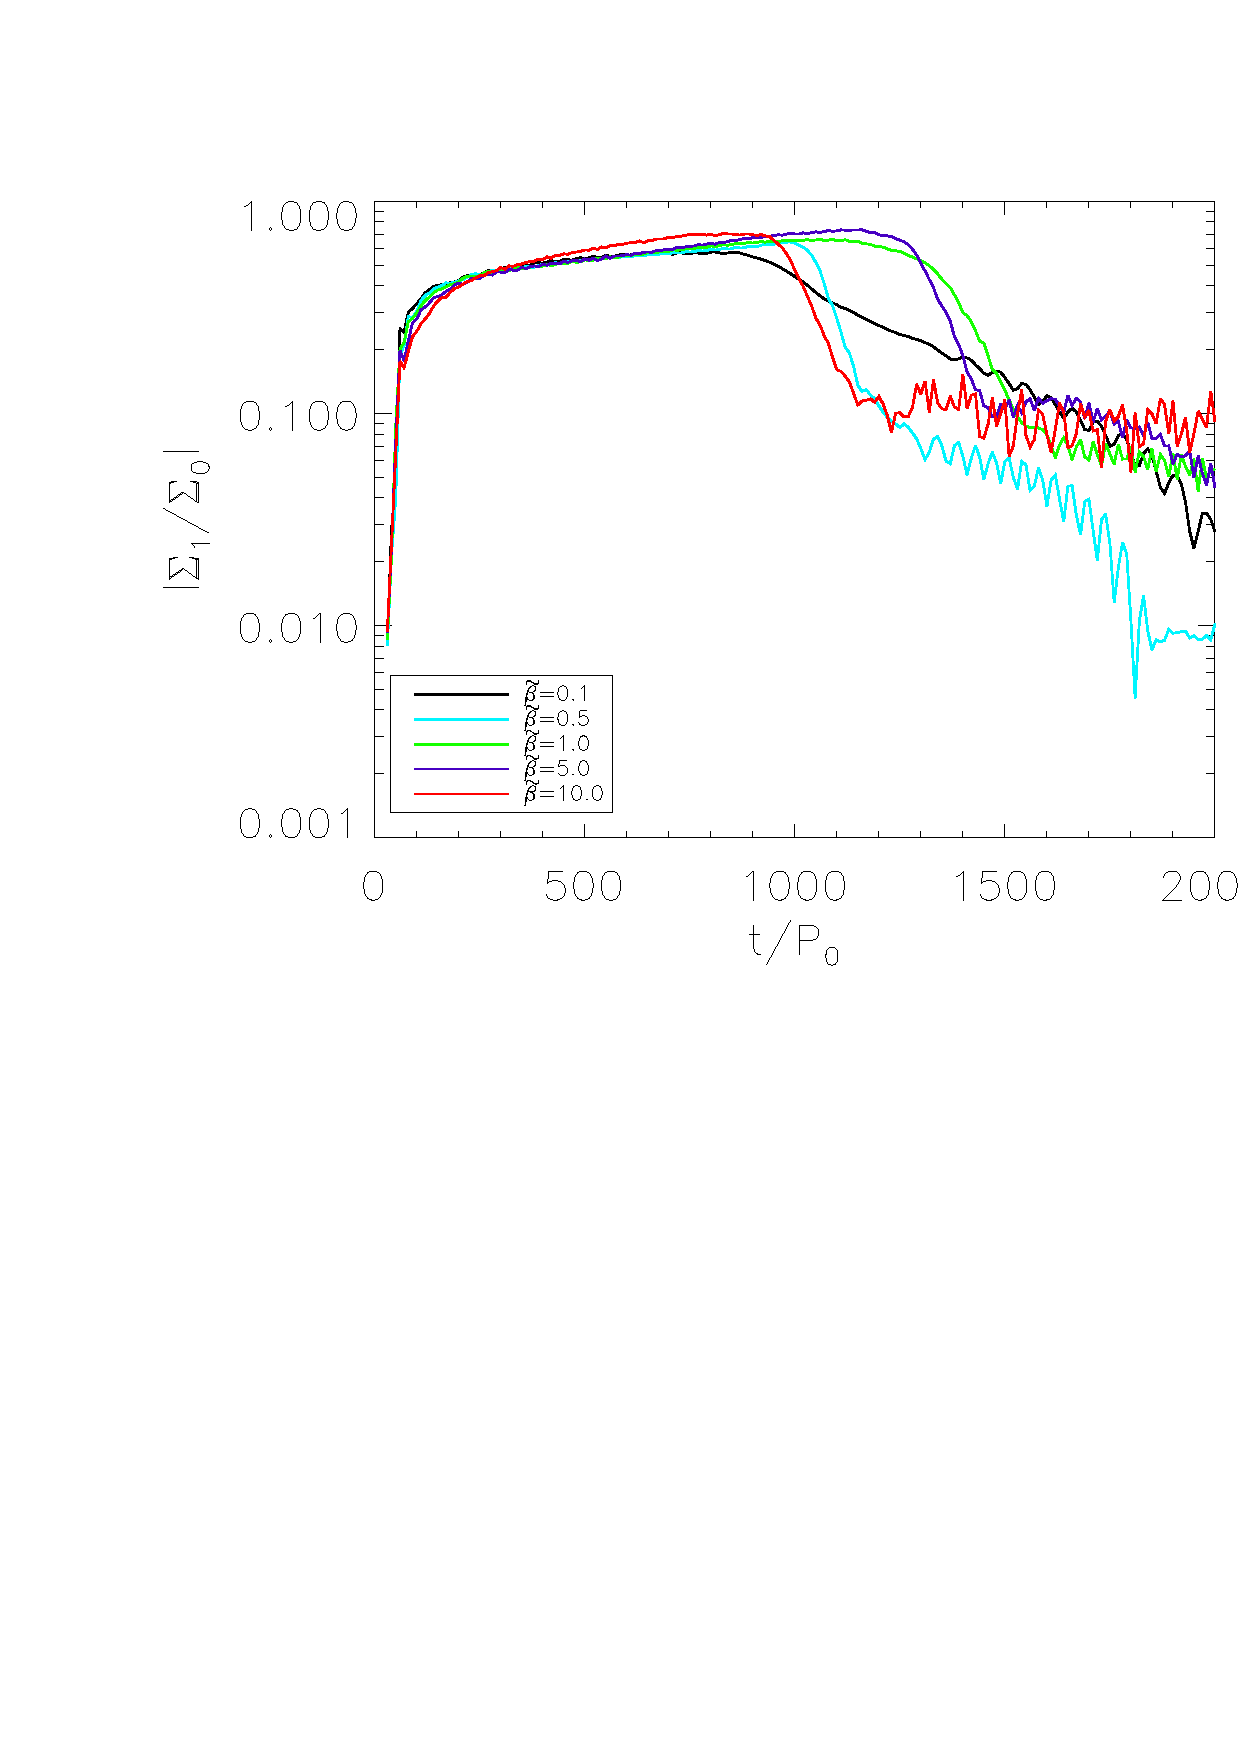
\includegraphics[width=\linewidth,clip=true,trim=0.5cm
    0cm 0cm 1cm]{figures/longterm_stability}
  \caption{Log plot of the $m=1$ mode non-dimenionlized by the $m=0$ background mode for longterm non-linear simulations corrsponding to vortex lifetime. The longest living mode correpsonds to $\tilde\beta=5.0$ (the red line). \label{lifetimeplot}}
\end{figure}

\begin{figure}
  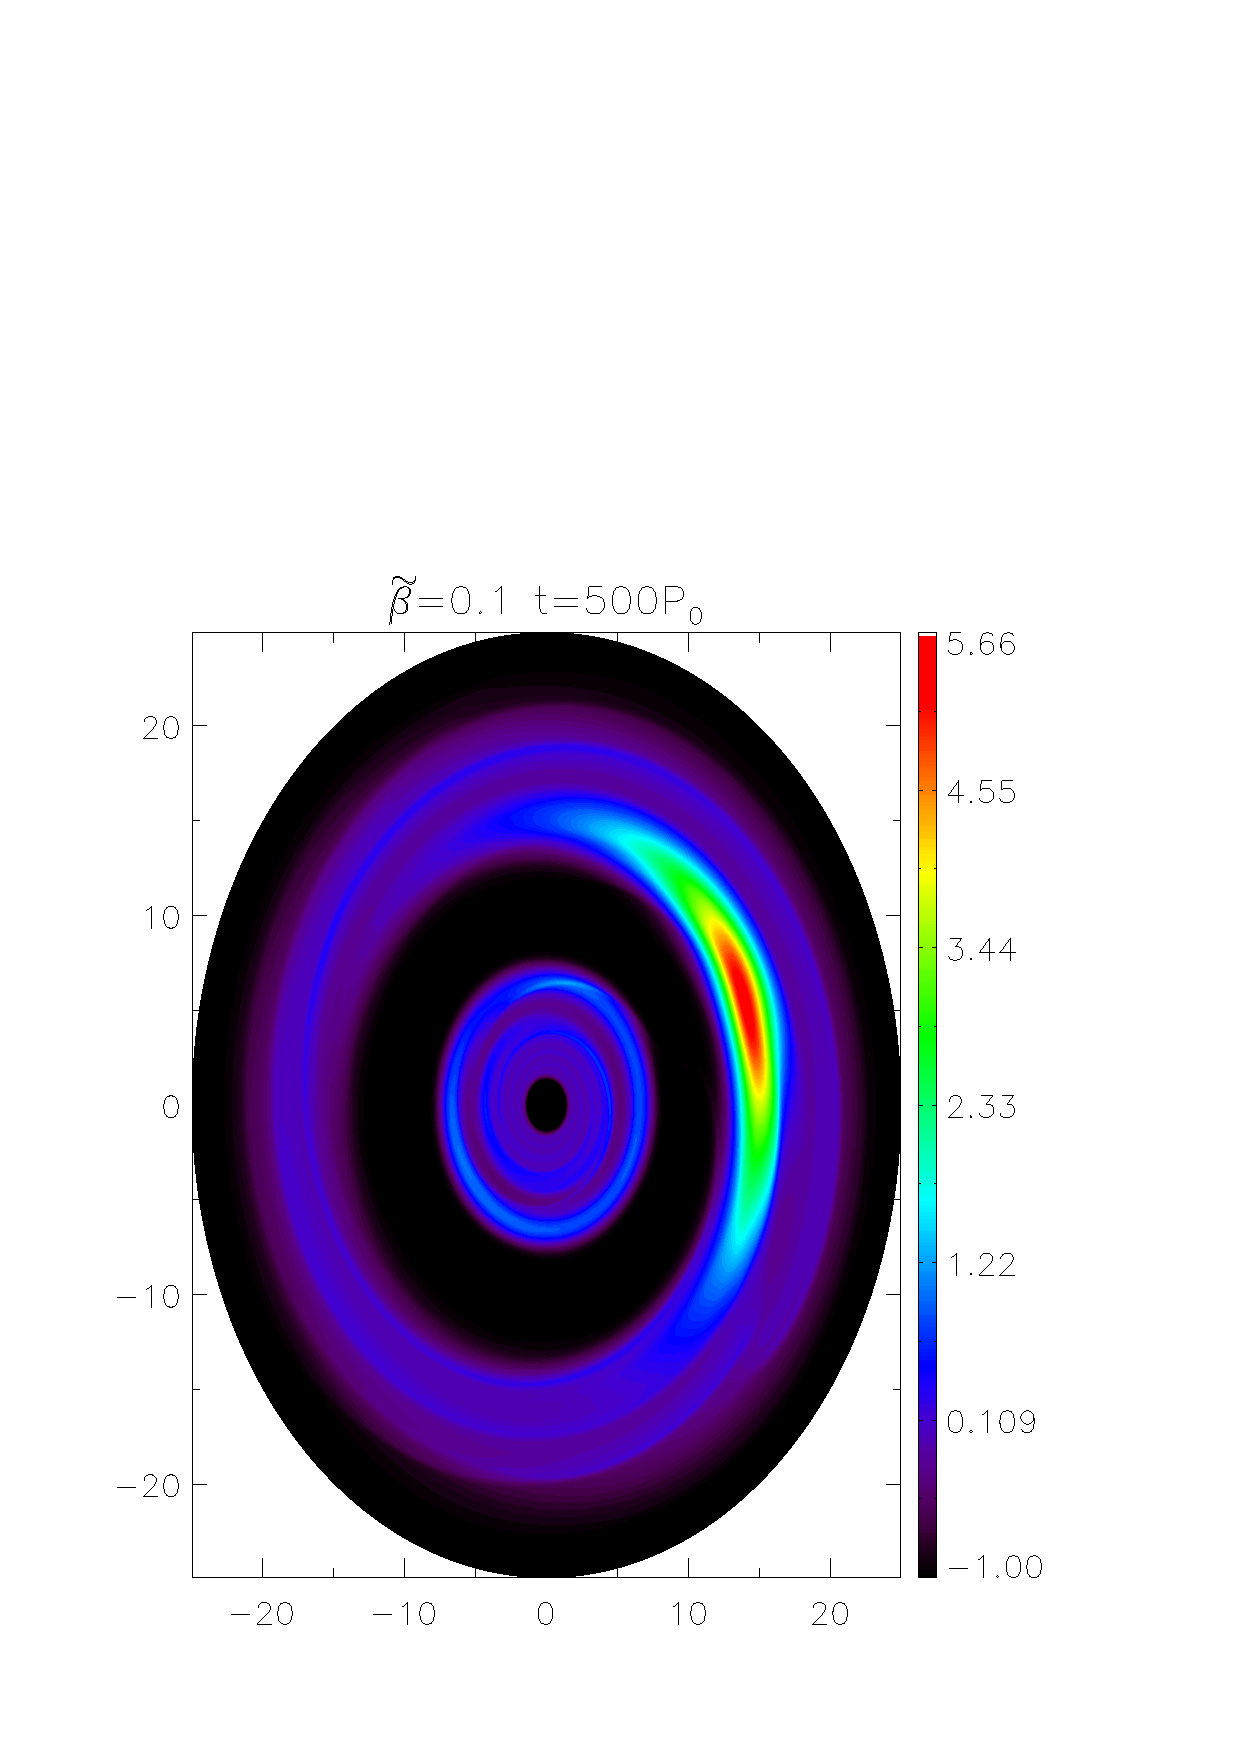
\includegraphics[width=\linewidth,height=\linewidth]{figures/vortex2D}
  \caption{Cartesian plot of relative density pertibation for $\tilde\beta=0.1$ vortex case during the quasi-steady state. The large scale non-axisyemetric $m=1$ overdensity can be seen. \label{Vortex2D}}
\end{figure}

%\begin{figure}
%   \includegraphics[scale=.42]{figures/stability_vis6betalow.ps}
%   \caption{Same as Fig. \ref{stability_vis9lowb} but $\hat{\nu}=10^{-6}$ and $\tilde{\beta}=0.1$. }
% \label{stability_vis6lowb)}
% \end{figure}

%\begin{figure}
%   \includegraphics[scale=.42]{figures/stability_vis6betamed.ps}
%   \caption{Same as Fig. \ref{stability_vis9lowb} but $\hat{\nu}=10^{-6}$ and $\tilde{\beta}=1.0$. }
% \label{stability_vis6medb)}
% \end{figure}
%Same as \ref{stability_vis9lowb} but $\hat{\nu}=10^{-6}$ and $\tilde{\beta}=1.0$. 


%we checked that open bc doesn't affect gap structure
%checked that t=200 plots are similar to t=100 

%surface density plot

%aspect-ratio plot

%general vortensity plot 



%% \begin{figure}
%%   \includegraphics[scale=.42,clip=true,trim=0cm 1.8cm 0cm 0cm]{figures/compare_profiles_dens020.ps}\\
%%   \includegraphics[scale=.42]{figures/compare_profiles_h020.ps}
%%   \caption{Steady-state gap profiles in a low mass viscous disc. The
%%     surface density perturbation (top) and disc aspect-ratio (bottom)
%%     are shown as a function of the cooling parameter:  
%%     $\tbeta=0.1$ (solid, fast cooling), $\tbeta=1$ (dotted,
%%     moderate cooling) and $\tbeta=10$ (dashed, slow
%%     cooling). \label{lvisc_steady_gap}}  
%% \end{figure}



%% \begin{figure}
%%   \includegraphics[scale=.42]{figures/compare_profiles_gvort020.ps}
%%   \caption{Gap structure in a low mass viscous disc, in terms of the
%%     perturbed generalized vortensity as a function of the cooling
%%     parameter. \label{lvisc_steady_gvort}} 
%% \end{figure}


%%\section{Gaps in massive discs (MKL)}
%% We first examine disc models with $Q_o=1.5$. We set the physical
%% viscosity $\hat{\nu}=10^{-9}$, so that the only energy source is
%% through shock-heating (via artificial viscosity) and the $\mathcal{C}$
%% function when $e\Sigma<e_i\Sigma_i$. The numerical resolution is
%% $N_r\times N_\phi = 512\times 1024$.   

%% %Since we are primarily concerened with gap stability, it is important
%% %to first examine the gap structured opened by the planet as a function
%% %of cooling. 
%% Fig. \ref{gvort1d_q1d5} compares the gap structure in terms of the GV profile for three
%% levels of cooling: $\tilde{\beta}=0.1$, $\tilde{\beta}=1$ and
%% $\tbeta=10$. For convenience we will refer to these cases as fast,
%% intermediate and slow cooling, respectively. The snapshot is taken at
%% $t=30P_0$, just after the planet is fully introduced. 

%% In terms of the GV profile, the qualitative features of the planetary
%% gap --- localized GV extrema at the gap edges --- remain unchanged
%% despite two orders of magnitude difference in the cooling rate.   


%% \begin{figure}
%% %  \includegraphics[scale=.42,clip=true,trim=0cm 1.8cm 0cm 0cm]{figures/dens1d_q1d5_003_global.ps}\\
%% %  \includegraphics[scale=.42]{figures/gvort1d_q1d5_003_global.ps}
%%   \caption{Gap structure in terms of the perturbed surface density
%%     (top) and perturbed generalized
%%     vortensity (bottom), as a function of the cooling parameter:  
%%     $\tbeta=0.1$ (solid, fast cooling), $\tbeta=1$ (dotted,
%%     intermediate cooling) and $\tbeta=10$ (dashed, slow
%%     cooling). \label{gvort1d_q1d5}} 
%% \end{figure}

%% \begin{figure*}
%% %  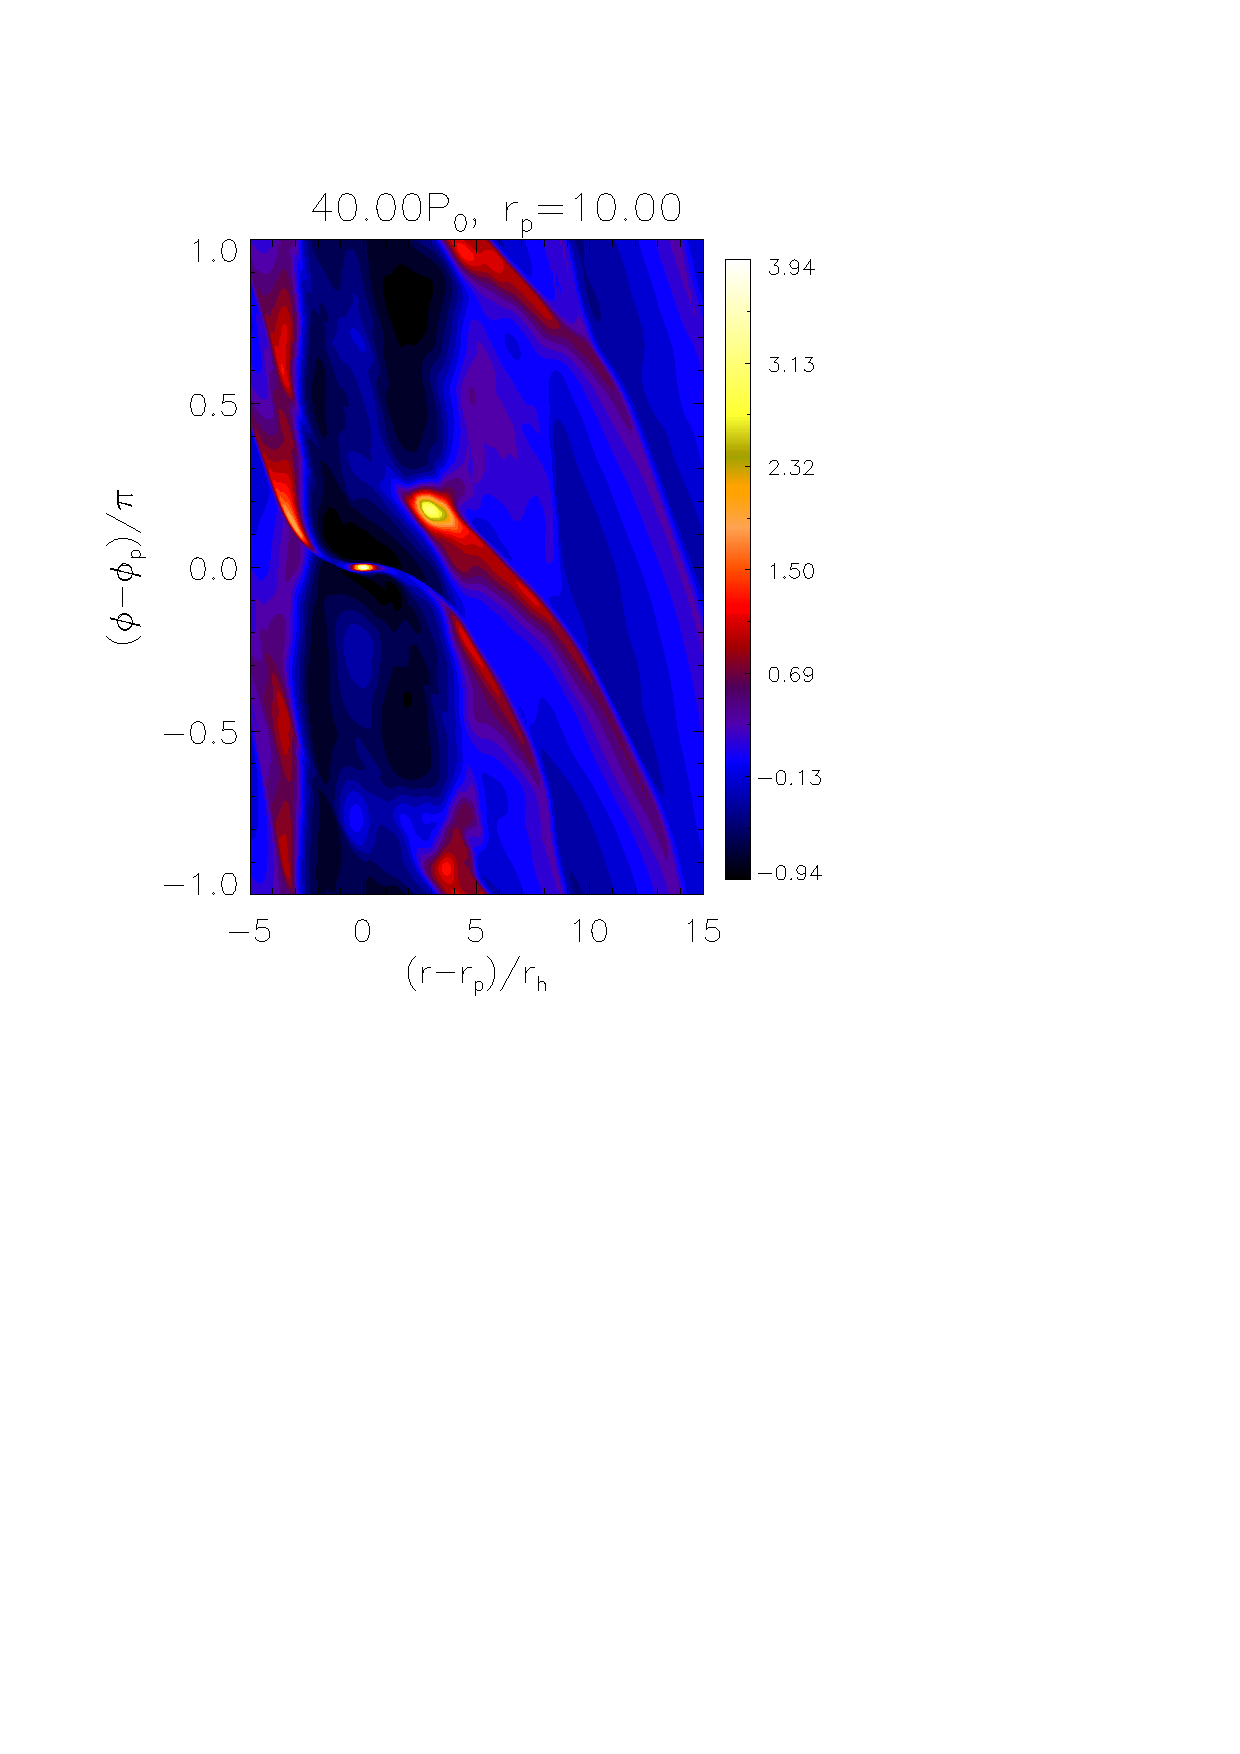
\includegraphics[scale=.55,clip=true,trim=0cm 0cm 0cm
%% %    0cm]{figures/noniso0_HR_dens004}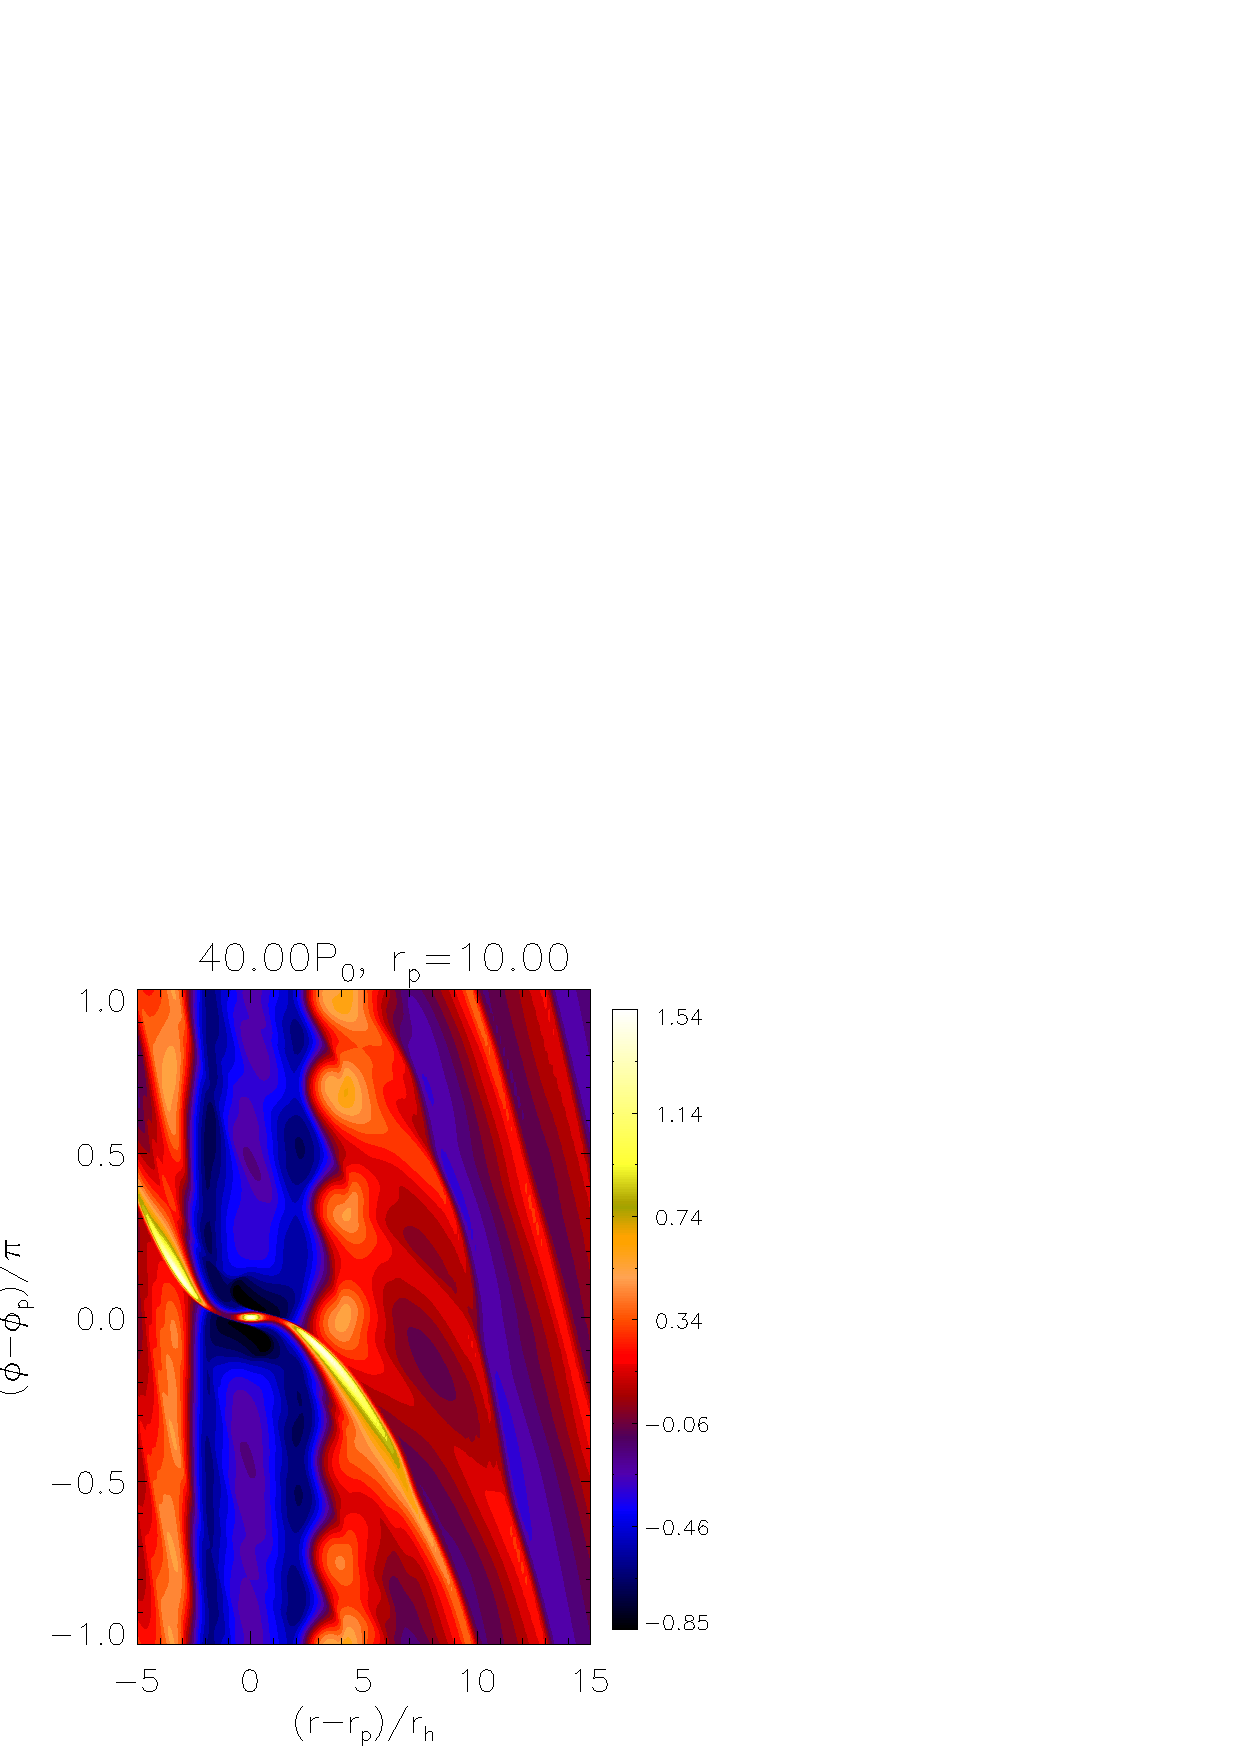
\includegraphics[scale=.55,clip=true,trim=2.26cm 0cm 0cm
%% %    0cm]{figures/noniso1_HR_dens004}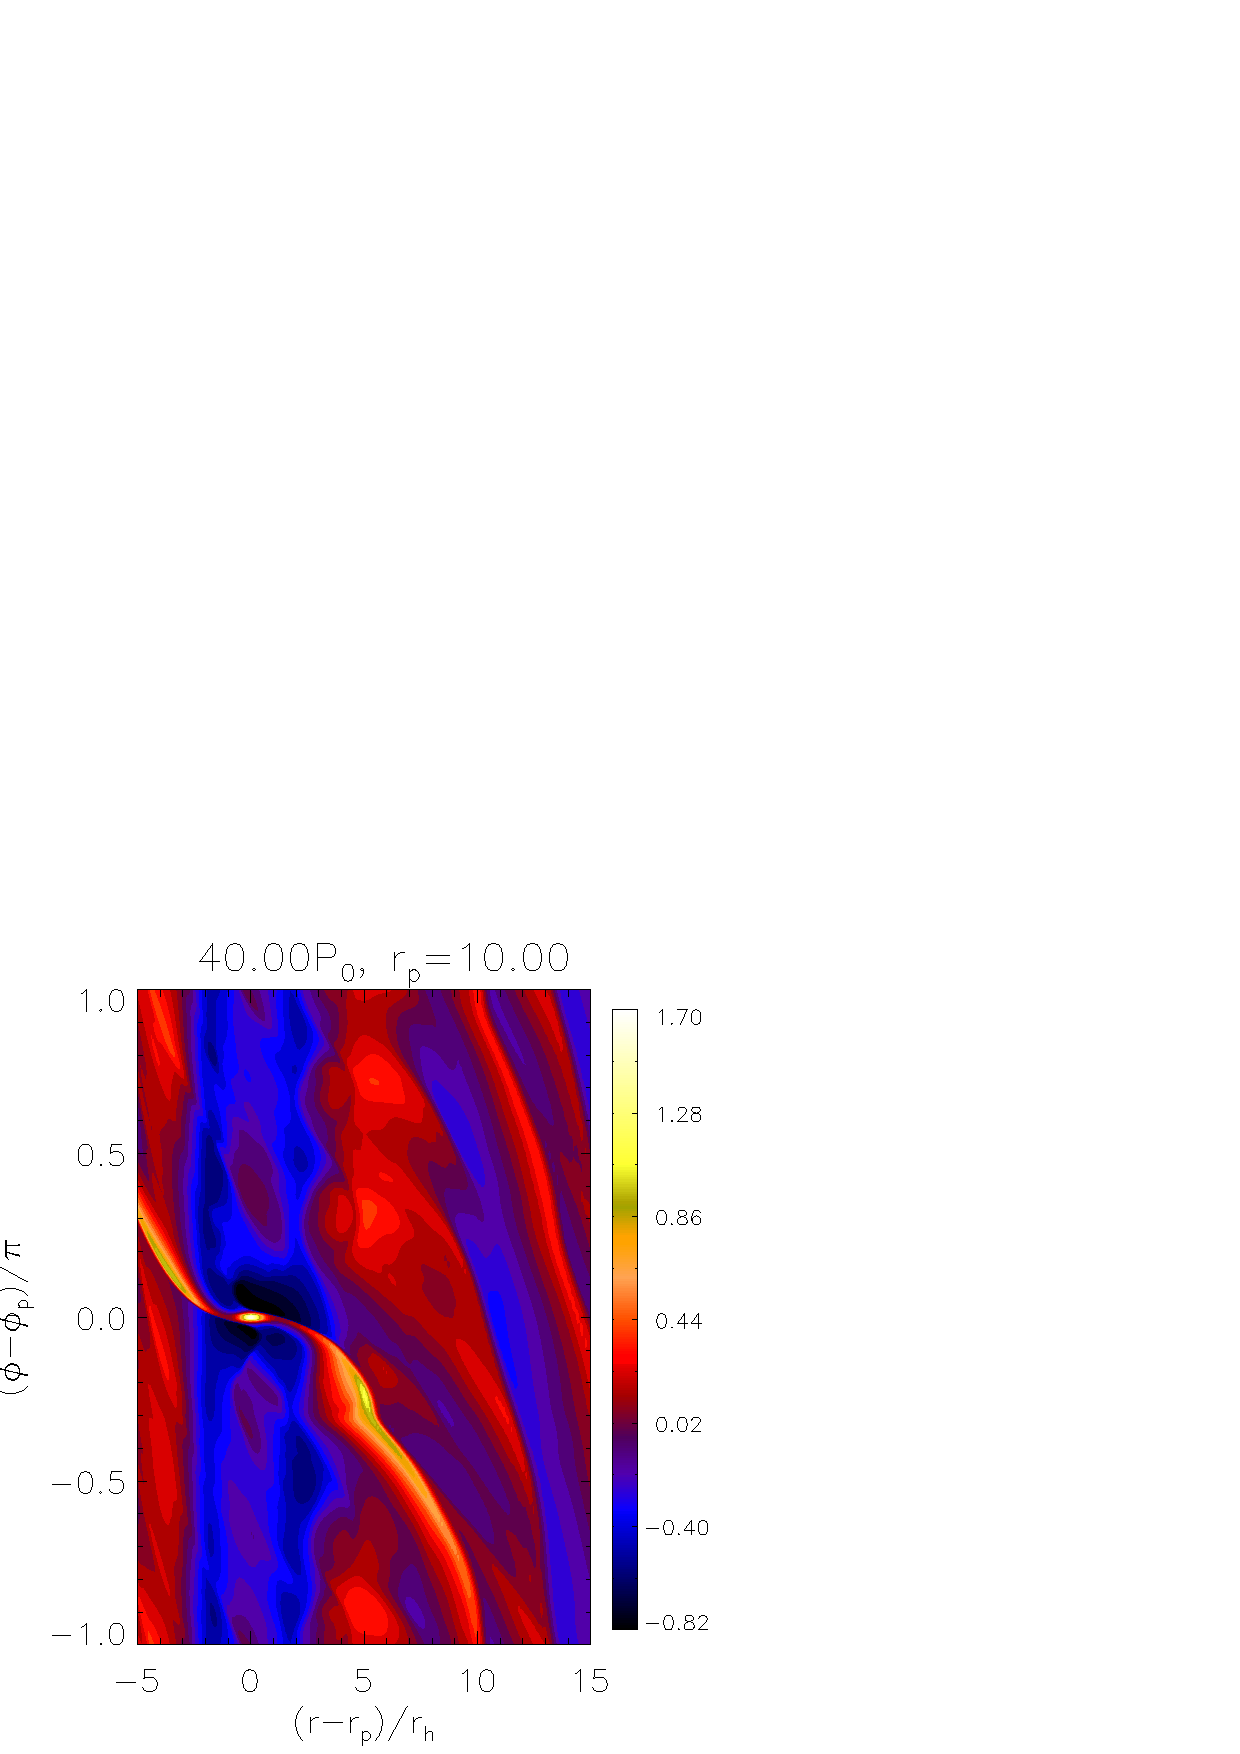
\includegraphics[scale=.55,clip=true,trim=2.26cm 0cm 0cm
%% %    0cm]{figures/noniso2_HR_dens004}
%%   \caption{Gap instability in the heavy disc model, as a function of
%%     the cooling parameter: $\tbeta=0.1$ (left), $\tbeta=1$ (middle)
%%     and $\tbeta=10$ (right). The relative surface density
%%     perturbation is shown. \label{polarxy_q1d5}} 
%% \end{figure*}
